\documentclass[conference]{IEEEtran}
\usepackage[utf8]{inputenc}
\usepackage{cite}
\usepackage{graphicx}
\usepackage{booktabs}
\usepackage{tabularx}
\usepackage{amsmath}
\usepackage{amssymb}
\usepackage{url}
\usepackage{xcolor}
\usepackage{tikz}
\usetikzlibrary{arrows.meta,positioning,shapes.geometric}
\usepackage{listings}
\lstset{basicstyle=\ttfamily\footnotesize,breaklines=true,frame=single,
        backgroundcolor=\color{gray!5},columns=fullflexible}
\renewcommand{\ttdefault}{cmtt}
\newcommand{\placeholder}[1]{\textcolor{red}{[\textbf{PLACEHOLDER: #1}]}}
\newcommand{\planned}{\textcolor{blue}{\textit{Planned implementation; not yet measured.}}}

\begin{document}
\title{Agentic Retrieval-Augmented Generation over a Financial Data Mart}
\author{\IEEEauthorblockN{Bhavani Patangay}
\IEEEauthorblockA{Department of Computer Science\\
Kennesaw State University\\
Marietta, U.S.A.\\
bpatanga@students.kennesaw.edu}}
\maketitle

\begin{abstract}
This project proposes an end-to-end analytical platform combining a PostgreSQL financial data mart, traditional machine-learning models, and an agentic retrieval-augmented generation (RAG) interface for Lending Club loan-performance analysis. The proposed dimensional model uses a central loan-performance fact table linked to borrower, loan, grade, and date dimensions. A temporal evaluation reports decision-tree classification and linear-regression results: the classifier achieves 0.8003 accuracy and 0.2002 recall on the 2018 holdout, while regression results are mixed against a mean baseline. A FastAPI/RAG service remains proposed; its implementation and benchmark are not verified here. This report distinguishes supplied model metrics from unverified end-to-end implementation and dataset artifacts.
\end{abstract}

\begin{IEEEkeywords}
Data warehousing, star schema, Lending Club, decision trees, linear regression, PostgreSQL, FastAPI, retrieval-augmented generation, text-to-SQL.
\end{IEEEkeywords}

\section{Introduction}
Financial institutions need to answer portfolio questions across many interacting dimensions, including loan grade, origination period, borrower income and debt profile, loan status, and repayment outcome. Conventional dashboards support predefined measures but can be inflexible for ad hoc business questions. The proposed system addresses this gap by separating analytical storage from natural-language interaction: PostgreSQL provides a dimensional data mart, scikit-learn provides interpretable and predictive models, and an agentic RAG workflow translates approved natural-language questions into executable SQL.

The target use cases include charge-off trend analysis, grade-level default risk, borrower-segment comparisons, expected recovery analysis, and portfolio concentration queries. The system is intended to provide both quantitative results and executive-readable explanations while preserving an auditable SQL path.

\section{Problem Statement}
Business stakeholders require ad hoc visibility into loan portfolio risk, charge-off trends, and credit exposure, but translating natural-language questions into multi-dimensional SQL requires technical expertise. Static reporting tools cannot readily adapt to changing analytical questions.

The project therefore asks: \emph{Can a PostgreSQL star schema, conventional machine-learning models, and schema-grounded RAG be integrated into a system that answers Lending Club portfolio questions accurately and transparently?} Success requires a dimensional model, reproducible ETL, auditable risk rules, useful aggregate results, safe text-to-SQL, and a benchmarked API. The scope is analytical decision support rather than approval of real consumers or automated credit decisions.

\section{Dataset and Selection}
\subsection{Data Source}
The proposed source is the public ``All Lending Club Loan Data'' dataset on Kaggle \cite{lendingclub}. The proposal specifies a subset of approximately 100,000 loan records originating between 2015 and 2018. The exact source release and CSV remain unverified in this checkout; the model-evaluation split is reported in Section~VII.

\subsection{Candidate Attributes}
Table~\ref{tab:data_attributes} summarizes candidate fields. Final data types and availability must be confirmed against the exact Kaggle release used.
\begin{table}[!t]
\caption{Candidate Lending Club Attributes}
\label{tab:data_attributes}
\centering
\begin{tabularx}{\columnwidth}{@{}l l X@{}}
\toprule
\textbf{Area} & \textbf{Attribute} & \textbf{Analytical use}\\
\midrule
Loan & loan\_amnt, int\_rate, term, installment & Exposure, pricing, payment burden\\
Grade & grade, sub\_grade & Risk segmentation and OLAP slicing\\
Borrower & annual\_inc, dti, revol\_util, fico\_range\_low & Risk and affordability features\\
Outcome & loan\_status & Define defaulted versus fully paid target\\
Recovery & total\_rec\_prncp & Recovery-oriented numerical outcome\\
Time & issue\_d, last\_pymnt\_d & Fact date keys and cohort trends\\
\bottomrule
\end{tabularx}
\end{table}

\subsection{Selection and Leakage Controls}
Records will be filtered by issue date and required fields, then divided for modeling with an appropriate train/test split. The status and post-issuance payment fields must not be included as predictors of an issue-time default model. Each modeling experiment will document feature selection and handling of missing values.

\section{Data Mart and Star Schema}
The proposed mart centers on \texttt{Fact\_Loan\_Performance}. Dimension keys support filtering and drill-down, and the fact grain is one Lending Club loan record.
\begin{table}[!t]
\caption{Proposed Star-Schema Grain and Measures}
\label{tab:star}
\centering
\begin{tabularx}{\columnwidth}{@{}l X@{}}
\toprule
\textbf{Object} & \textbf{Description}\\
\midrule
\texttt{Fact\_Loan\_Performance} & One row per loan; foreign keys and additive/non-additive measures\\
\texttt{Dim\_Date} & Issue year, quarter, month, and date attributes\\
\texttt{Dim\_Borrower} & Annual income, DTI, revolving utilization, FICO band, and surrogate key\\
\texttt{Dim\_Loan\_Grade} & Grade and sub-grade hierarchy\\
\texttt{Dim\_Loan} & Term, amount, interest rate, and installment; \planned\\
\bottomrule
\end{tabularx}
\end{table}

\begin{figure}[!t]
\centering
\resizebox{\columnwidth}{!}{%
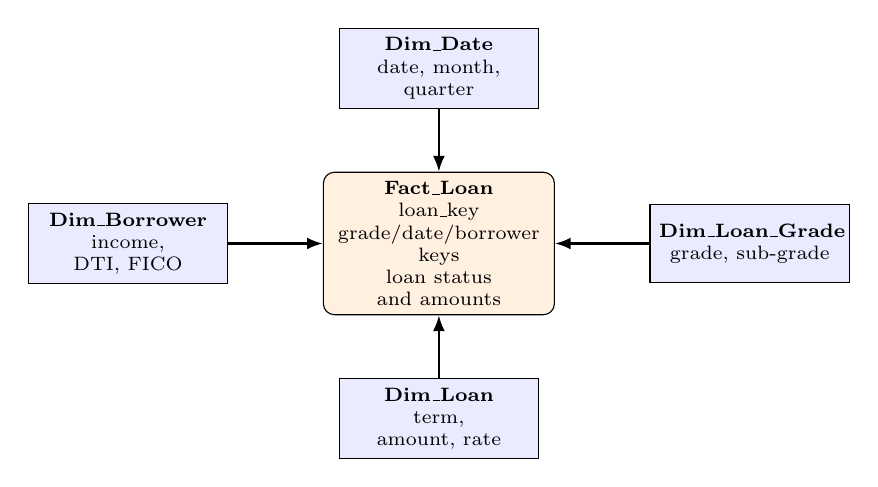
\begin{tikzpicture}[node distance=6mm, every node/.style={font=\scriptsize},
  fact/.style={rectangle,draw,rounded corners,fill=orange!12,text width=27mm,minimum height=12mm,align=center},
  dim/.style={rectangle,draw,fill=blue!8,text width=23mm,minimum height=10mm,align=center},
  arrow/.style={-{Latex[length=2mm]},thick}]
\node[fact] (fact) {\textbf{Fact\_Loan}\\loan\_key\\grade/date/borrower keys\\loan status and amounts};
\node[dim,left=12mm of fact] (borrower) {\textbf{Dim\_Borrower}\\income, DTI, FICO};
\node[dim,above=8mm of fact] (date) {\textbf{Dim\_Date}\\date, month, quarter};
\node[dim,right=12mm of fact] (grade) {\textbf{Dim\_Loan\_Grade}\\grade, sub-grade};
\node[dim,below=8mm of fact] (loan) {\textbf{Dim\_Loan}\\term, amount, rate};
\draw[arrow] (borrower)--(fact); \draw[arrow] (date)--(fact);
\draw[arrow] (grade)--(fact); \draw[arrow] (loan)--(fact);
\end{tikzpicture}}
\caption{Proposed star schema (ER-style schema diagram).}
\label{fig:star}
\end{figure}

\subsection{Data Dictionary}
Table~\ref{tab:dictionary} defines the conceptual fact and key dimensions. Surrogate keys are recommended to isolate the fact table from source identifiers and permit slowly changing dimensions.
\begin{table*}[!t]
\caption{Conceptual Data-Mart Data Dictionary}
\label{tab:dictionary}
\centering
\small
\begin{tabular}{@{}llllp{6.5cm}@{}}
\toprule
\textbf{Table} & \textbf{Column} & \textbf{Type} & \textbf{Key/Null} & \textbf{Definition}\\
\midrule
Fact & loan\_key & BIGINT & PK, NN & Loan surrogate key\\
Fact & borrower\_key & BIGINT & FK, NN & Reference to Dim\_Borrower\\
Fact & grade\_key & BIGINT & FK, NN & Reference to Dim\_Loan\_Grade\\
Fact & issue\_date\_key & INTEGER & FK, NN & YYYYMMDD key to Dim\_Date\\
Fact & loan\_amnt & NUMERIC & NN & Funded principal amount\\
Fact & status & VARCHAR & NN & Paid or charged-off analytic status\\
Fact & total\_rec\_prncp & NUMERIC & Nullable & Principal received, used for recovery analysis\\
Dim\_Borrower & annual\_inc & NUMERIC & Nullable & Reported annual income\\
Dim\_Borrower & dti & NUMERIC & Nullable & Debt-to-income ratio\\
Dim\_Borrower & fico\_range\_low & INTEGER & Nullable & Lower bound of FICO range\\
Dim\_Loan\_Grade & grade & CHAR(1) & NN & Lending Club loan grade\\
Dim\_Date & date\_key & INTEGER & PK & YYYYMMDD surrogate representation\\
\bottomrule
\end{tabular}
\end{table*}

\section{Data Preparation and ETL}
The proposed pipeline is: extract the selected CSV release; profile missing values and distributions; normalize status labels; convert dates and percentages; deduplicate records; generate dimension surrogate keys; load dimensions; and load the fact table transactionally. Pandas supports profiling and transformation, psycopg2 or SQLAlchemy provides PostgreSQL access, and staging tables should retain load-batch metadata.

Validation controls include source-versus-target row counts, null rejection for required keys, referential-integrity checks, date-range checks, duplicate loan keys, and reconciliation of loan principal sums. \planned

\section{Proposed Architecture}
The architecture comprises a presentation/API layer, RAG orchestration, retrieval of schema and approved SQL context, warehouse execution, traditional ML components, and an analytical frontend or API client.
\begin{figure*}[!t]
\centering
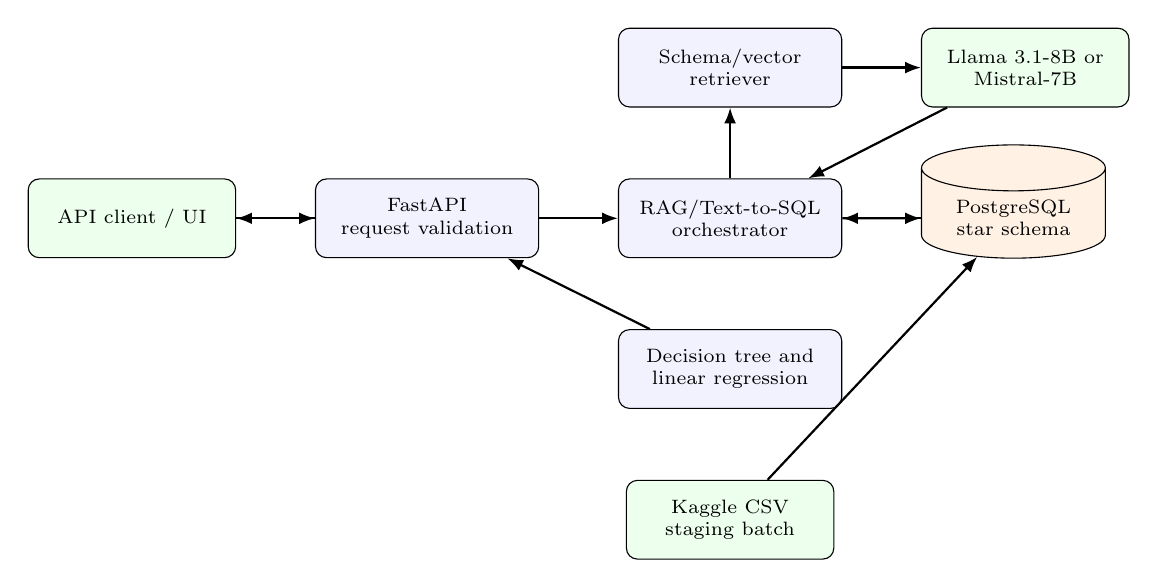
\begin{tikzpicture}[node distance=8mm, every node/.style={font=\scriptsize},
  component/.style={rectangle,draw,rounded corners,fill=blue!5,text width=26mm,minimum height=10mm,align=center},
  external/.style={rectangle,draw,rounded corners,fill=green!7,text width=24mm,minimum height=10mm,align=center},
  store/.style={cylinder,draw,shape border rotate=90,aspect=.25,fill=orange!10,text width=21mm,align=center,minimum height=13mm},
  arrow/.style={-{Latex[length=2mm]},thick}]
\node[external] (ui) {API client / UI};
\node[component,right=10mm of ui] (api) {FastAPI\\request validation};
\node[component,right=10mm of api] (rag) {RAG/Text-to-SQL\\orchestrator};
\node[component,above=9mm of rag] (retriever) {Schema/vector\\retriever};
\node[external,right=10mm of retriever] (llm) {Llama 3.1-8B or\\Mistral-7B};
\node[store,right=10mm of rag] (pg) {PostgreSQL\\star schema};
\node[component,below=9mm of rag] (ml) {Decision tree and\\linear regression};
\node[external,below=9mm of ml] (data) {Kaggle CSV\\staging batch};
\draw[arrow] (ui)--(api); \draw[arrow] (api)--(rag);
\draw[arrow] (rag)--(retriever); \draw[arrow] (retriever)--(llm);
\draw[arrow] (llm)--(rag); \draw[arrow] (rag)--(pg);
\draw[arrow] (pg)--(rag); \draw[arrow] (api)--(ui);
\draw[arrow] (data)--(pg); \draw[arrow] (ml)--(api);
\end{tikzpicture}
\caption{Proposed system architecture.}
\label{fig:architecture}
\end{figure*}

\subsection{Workflow and Sequence}
Figure~\ref{fig:sequence} shows the no-fabrication control flow. SQL must be generated from retrieved schema context, validated against an allowlist of read-only statements and table/column names, executed with limits, and summarized only after results exist.
\begin{figure}[!t]
\centering
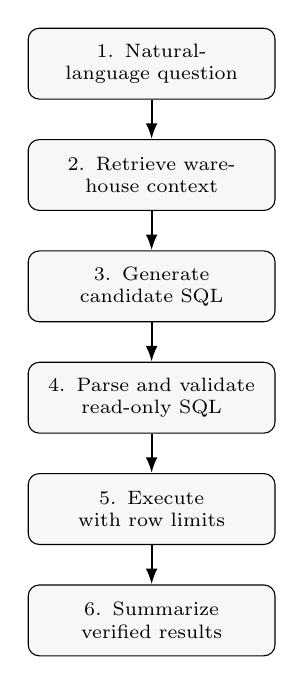
\begin{tikzpicture}[node distance=5mm, every node/.style={font=\scriptsize,rectangle,draw,rounded corners,fill=gray!6,text width=29mm,minimum height=9mm,align=center}]
\node (q) {1. Natural-language question};
\node[below=of q] (r) {2. Retrieve warehouse context};
\node[below=of r] (s) {3. Generate candidate SQL};
\node[below=of s] (v) {4. Parse and validate read-only SQL};
\node[below=of v] (e) {5. Execute with row limits};
\node[below=of e] (a) {6. Summarize verified results};
\draw[-{Latex[length=2mm]},thick] (q)--(r); \draw[-{Latex[length=2mm]},thick] (r)--(s); \draw[-{Latex[length=2mm]},thick] (s)--(v);
\draw[-{Latex[length=2mm]},thick] (v)--(e); \draw[-{Latex[length=2mm]},thick] (e)--(a);
\end{tikzpicture}
\caption{Text-to-SQL RAG workflow.}
\label{fig:sequence}
\end{figure}

\section{Machine Learning Models and Metrics}
\subsection{Decision-Tree Default Classification}
A decision tree \cite{hastie} was evaluated for distinguishing fully paid from charged-off loans. The temporal split trains on 93,642 loans from 2015--2017 and evaluates on an untouched 2018 holdout of 6,358 loans. The classification threshold, 0.397727, was selected by maximizing out-of-fold (OOF) recall subject to an OOF-accuracy floor of 77\%; at that threshold, training OOF accuracy is 0.7714, recall is 0.2303, and $F_1$ is 0.3075. The confusion matrix below lists rows as actual negative/positive and columns as predicted negative/positive.
\begin{align}
\text{Precision} &= \frac{TP}{TP+FP},\\
\text{Recall} &= \frac{TP}{TP+FN},\\
F_1 &= \frac{2TP}{2TP+FP+FN},\\
\text{Accuracy} &= \frac{TP+TN}{TP+TN+FP+FN}.
\end{align}
\begin{table*}[!t]
\caption{Temporal-Holdout Default-Classification Results}
\label{tab:classification_results}
\centering
\footnotesize
\renewcommand{\arraystretch}{0.9}
\begin{tabularx}{\textwidth}{@{}Xrrr@{}}
\toprule
\textbf{Measure} & \textbf{Tuned (0.397727)} & \textbf{Majority} & \textbf{Prior max-$F_1$ (0.229)}\\
\midrule
2018 accuracy & 0.8003 & 0.8413 & 0.6291\\
2018 precision & 0.3038 & --- & ---\\
2018 recall & 0.2002 & 0 & 0.6571\\
2018 $F_1$ & 0.2413 & 0 & 0.3599\\
2018 ROC-AUC & 0.6869 & 0.5000 & ---\\
2018 AP (PR-AUC) & 0.2671 & 0.1587 & ---\\
Confusion matrix & $[[4886,463],[807,202]]$ & --- & ---\\
\bottomrule
\end{tabularx}
\end{table*}
The selected threshold trades some accuracy for positive-class detection relative to the majority baseline, but recall remains modest. The earlier max-$F_1$ threshold has higher recall and $F_1$ but substantially lower accuracy; these operating points show the accuracy--recall tradeoff, not overall superiority. The proposal's numeric threshold-compliance criterion has not been verified and is not claimed.

\subsection{Linear Recovery Regression}
Linear regression \cite{scikitlearn} was evaluated for a recovery-related outcome against a mean-prediction baseline. The mean squared error (MSE) and coefficient of determination ($R^2$) are:
\begin{align}
\mathrm{MSE} &= \frac{1}{n}\sum_{i=1}^{n}(y_i-\hat y_i)^2, &
R^2 &= 1-\frac{\sum_i(y_i-\hat y_i)^2}{\sum_i(y_i-\bar y)^2}.
\end{align}
\begin{table}[!t]
\caption{Recovery-Regression Results}
\label{tab:regression_results}
\centering
\small
\begin{tabularx}{\columnwidth}{@{}Xrr@{}}
\toprule
\textbf{Measure} & \textbf{Linear regression} & \textbf{Mean baseline}\\
\midrule
MAE & 3011.69 & 3156.40\\
RMSE & 3796.35 & 3464.18\\
$R^2$ & $-3.311$ & $-2.589$\\
\bottomrule
\end{tabularx}
\end{table}
The model has lower MAE but higher RMSE and a more negative $R^2$ than the baseline, indicating a weak, mixed fit rather than overall improvement.

\subsection{Model Outputs}
The tree should expose depth, impurity, split thresholds, feature importance, and a text or graph representation to support auditable rules. The linear model should report coefficients and residual diagnostics. Scaling and encoding must be performed through a pipeline fitted only on training data.

\section{RAG/Text-to-SQL Methodology}
The RAG knowledge base is DDL-oriented context rather than a vector store of financial records alone. It contains table descriptions, relationships, data types, sample approved queries, and metric definitions. Retrieval should use the user's question to select relevant context. The model is instructed to generate one SQL statement, avoid data modification, qualify tables, and return only a SQL code block or a no-answer state.

The benchmark will contain 40 natural-language questions from the proposal. For each, the report can record syntax success, schema entity match, result-set exactness, and latency:
\begin{align}
\text{SQL success} &= \frac{\#\text{ executable read-only queries}}{\#\text{ attempts}},\\
\text{Entity match} &= \frac{\#\text{ correct referenced tables/columns}}{\#\text{ required entities}},\\
\text{Latency} &= t_{\text{response}}-t_{\text{request}}.
\end{align}
The 40-query set, model deployment, and measurements are \planned. Result-set match should compare normalized rows and column names, not SQL string equality.

\section{Implementation and API/UI}
\subsection{Technology}
The proposed implementation uses FastAPI \cite{fastapi}, PostgreSQL, Python, pandas, psycopg2 or SQLAlchemy, and scikit-learn \cite{scikitlearn}. NRP GPU execution may use an open-weight model only as capacity permits. The project should remain usable by replacing the local model endpoint or by running a deterministic text-to-SQL fallback.

\subsection{Repository Layout}
\begin{lstlisting}
docs/report.tex
docs/report.md
docs/report.pdf
lending_club/
tests/test_lending_club.py
pyproject.toml
data/             # Local-only and Git-ignored
artifacts/        # Local-only and Git-ignored
\end{lstlisting}

\subsection{Setup Commands}
\begin{lstlisting}
python3 -m venv .venv
source .venv/bin/activate
python -m pip install -e .
python -m lending_club.cli prepare /external/path.csv data/loans.csv
python -m lending_club.cli load data/loans.csv data/lending_club.db
python -m lending_club.cli train data/loans.csv artifacts/
uvicorn lending_club.api:app --reload
\end{lstlisting}
\subsection{Example Analytical Queries}
\begin{lstlisting}
What is the total loan amount charged off by loan grade in 2017?
Show the quarterly trend of fully paid and charged-off loans.
Which FICO bands have the highest charge-off rate?
What principal was recovered by grade and issue year?
\end{lstlisting}
Each response should include generated SQL, row count, and an abbreviated interpretation. Prompted schema entities must be checked before execution.

\section{Experimental Setup and Results}
\subsection{Proposed Experimental Setup}
The dataset is partitioned into issue-date cohorts and a held-out test partition. ETL, training, and RAG configurations are to be recorded in a machine-readable configuration or seed file. Experiments should report package versions, split definition, random seeds, PostgreSQL version, hardware, model name, model quantization, and API latency conditions.

\subsection{Results Status}
The temporal model evaluation summary provides classification and regression metrics reported in Tables~\ref{tab:classification_results} and~\ref{tab:regression_results}. The underlying Kaggle CSV, model artifact, execution log, and full implementation are not present in the inspected worktree, so those results cannot be independently reproduced from this checkout. The RAG benchmark and full API/data-mart implementation remain unverified. Table~\ref{tab:status} distinguishes reported model results from missing artifacts.
\begin{table}[!t]
\caption{Evidence and Experimental-Result Status}
\label{tab:status}
\centering
\small
\renewcommand{\arraystretch}{0.9}
\begin{tabularx}{\columnwidth}{@{}p{0.40\columnwidth}X@{}}
\toprule
\textbf{Item} & \textbf{Verified status}\\
\midrule
Dataset source & Proposed by project proposal\\
Model split & 93,642 train; 6,358 holdout (2018)\\
Classifier results & See Table~\ref{tab:classification_results}\\
Regression results & See Table~\ref{tab:regression_results}\\
Raw data/artifacts & \placeholder{not present for reproduction}\\
PostgreSQL schema & \placeholder{not implemented}\\
40-query benchmark & \placeholder{not implemented}\\
FastAPI service & \placeholder{not implemented}\\
\bottomrule
\end{tabularx}
\end{table}

\section{Evaluation}
Evaluation combines three complementary views: warehouse correctness, model validity, and RAG usefulness. Warehouse correctness still requires reconciliations and referential checks. The reported temporal model results show a classifier threshold tradeoff and mixed recovery-regression performance against a mean baseline; underlying files are needed for independent reproduction. RAG usefulness still requires measuring SQL correctness and latency; human judgments should be separated from automatic metrics.

Recommended baseline comparisons are:
\begin{itemize}
\item Majority-class and logistic-regression baselines for default classification;
\item Mean-target and ordinary linear regression baselines for recovery;
\item direct rule-based SQL versus schema-grounded text-to-SQL;
\item prompt-only SQL versus retrieval-augmented SQL.
\end{itemize}

\section{Limitations and Future Work}
The public Kaggle source may contain historical, incomplete, or inconsistent labels. The 2015--2018 subset is a convenience sample and may not represent current consumer behavior or other lenders. Missing data, class imbalance, and survivorship effects can bias classification. Aggregate patterns must not be interpreted as individualized credit decisions.

LLM generated SQL can hallucinate fields or produce semantically plausible but incorrect queries. Read-only execution, statement allowlisting, row limits, timeout, SQL parsing, and human review mitigate these risks. Retrieval can reduce errors but cannot guarantee correctness.

Future work should add incremental ETL, slowly changing dimensions, tests for SQL and metric calculations, dashboards, retrieval evaluation, confidence reporting, query cancellation, audit logs, model monitoring, and an explicit fairness/bias analysis. An assignment of real-world LGD or life of loan values should require domain validation.

\section{Conclusion}
The proposal defines a coherent financial data-mart and agentic RAG project, with a star schema for OLAP-style analysis and a proposed FastAPI interface. The supplied temporal evaluation reports measurable but qualified model results: the selected decision threshold favors an accuracy constraint over higher recall, while recovery regression improves MAE but not RMSE or $R^2$ versus the mean baseline. The full data mart, API, RAG benchmark, and raw artifacts remain unverified in the inspected checkout; the model metrics therefore require their source artifacts for independent reproduction.

\begin{thebibliography}{00}
\bibitem{lendingclub}{N. George, ``All Lending Club Loan Data,'' Kaggle, 2019. [Online]. Available: https://www.kaggle.com/datasets/wordsforthewise/lending-club}
\bibitem{rag}{P. Lewis \emph{et al.}, ``Retrieval-augmented generation for knowledge-intensive NLP tasks,'' in \emph{Advances in Neural Information Processing Systems}, 2020, pp. 9459--9474.}
\bibitem{hastie}{T. Hastie, R. Tibshirani, and J. Friedman, \emph{The Elements of Statistical Learning}, 2nd ed. New York, NY, USA: Springer, 2009.}
\bibitem{scikitlearn}{F. Pedregosa \emph{et al.}, ``Scikit-learn: Machine learning in Python,'' \emph{J. Machine Learning Research}, vol. 12, pp. 2825--2830, 2011.}
\bibitem{fastapi}{S. Ram\'{i}rez, ``FastAPI,'' 2018. [Online]. Available: https://fastapi.tiangolo.com/}
\bibitem{kimball}{R. Kimball and M. Ross, \emph{The Data Warehouse Toolkit}, 3rd ed. Indianapolis, IN, USA: Wiley, 2013.}
\bibitem{postgres}{The PostgreSQL Global Development Group, ``PostgreSQL Documentation.'' [Online]. Available: https://www.postgresql.org/docs/}
\bibitem{llama}{Meta AI, ``Llama 3.1 Model Card,'' 2024. [Online]. Available: https://llama.meta.com/}
\bibitem{textsql}{A. Rajkumar \emph{et al.}, ``Evaluating text-to-SQL capabilities of large language models,'' arXiv:2204.00498, 2022.}
\end{thebibliography}
\end{document}
